\iffalse
\let\negmedspace\undefined
\let\negthickspace\undefined
\documentclass[journal,12pt,onecolumn]{IEEEtran}
\usepackage{cite}
\usepackage{amsmath,amssymb,amsfonts,amsthm}
\usepackage{algorithmic}
\usepackage{graphicx}
\usepackage{textcomp}
\usepackage{xcolor}
\usepackage{txfonts}
\usepackage{listings}
\usepackage{enumitem}
\usepackage{mathtools}
\usepackage{gensymb}

\usepackage{tkz-euclide} % loads  TikZ and tkz-base
\usepackage{listings}



\newtheorem{theorem}{Theorem}[section]
\newtheorem{problem}{Problem}
\newtheorem{proposition}{Proposition}[section]
\newtheorem{lemma}{Lemma}[section]
\newtheorem{corollary}[theorem]{Corollary}
\newtheorem{example}{Example}[section]
\newtheorem{definition}[problem]{Definition}
%\newtheorem{thm}{Theorem}[section] 
%\newtheorem{defn}[thm]{Definition}
%\newtheorem{algorithm}{Algorithm}[section]
%\newtheorem{cor}{Corollary}
\newcommand{\BEQA}{\begin{eqnarray}}
\newcommand{\EEQA}{\end{eqnarray}}
\newcommand{\system}[1]{\stackrel{#1}{\rightarrow}}

\newcommand{\define}{\stackrel{\triangle}{=}}
\theoremstyle{remark}
\newtheorem{rem}{Remark}
%\bibliographystyle{ieeetr}
\begin{document}
%
\providecommand{\pr}[1]{\ensuremath{\Pr\left(#1\right)}}
\providecommand{\prt}[2]{\ensuremath{p_{#1}^{\left(#2\right)} }}        % own macro for this question
\providecommand{\qfunc}[1]{\ensuremath{Q\left(#1\right)}}
\providecommand{\sbrak}[1]{\ensuremath{{}\left[#1\right]}}
\providecommand{\lsbrak}[1]{\ensuremath{{}\left[#1\right.}}
\providecommand{\rsbrak}[1]{\ensuremath{{}\left.#1\right]}}
\providecommand{\brak}[1]{\ensuremath{\left(#1\right)}}
\providecommand{\lbrak}[1]{\ensuremath{\left(#1\right.}}
\providecommand{\rbrak}[1]{\ensuremath{\left.#1\right)}}
\providecommand{\cbrak}[1]{\ensuremath{\left\{#1\right\}}}
\providecommand{\lcbrak}[1]{\ensuremath{\left\{#1\right.}}
\providecommand{\rcbrak}[1]{\ensuremath{\left.#1\right\}}}
\newcommand{\sgn}{\mathop{\mathrm{sgn}}}
\providecommand{\abs}[1]{\left\vert#1\right\vert}
\providecommand{\res}[1]{\Res\displaylimits_{#1}} 
\providecommand{\norm}[1]{\left\lVert#1\right\rVert}
%\providecommand{\norm}[1]{\lVert#1\rVert}
\providecommand{\mtx}[1]{\mathbf{#1}}
\providecommand{\mean}[1]{E\left[ #1 \right]}
\providecommand{\cond}[2]{#1\middle|#2}
\providecommand{\fourier}{\overset{\mathcal{F}}{ \rightleftharpoons}}
\newenvironment{amatrix}[1]{%
  \left(\begin{array}{@{}*{#1}{c}|c@{}}
}{%
  \end{array}\right)
}
%\providecommand{\hilbert}{\overset{\mathcal{H}}{ \rightleftharpoons}}
%\providecommand{\system}{\overset{\mathcal{H}}{ \longleftrightarrow}}
	%\newcommand{\solution}[2]{\textbf{Solution:}{#1}}
\newcommand{\solution}{\noindent \textbf{Solution: }}
\newcommand{\cosec}{\,\text{cosec}\,}
\providecommand{\dec}[2]{\ensuremath{\overset{#1}{\underset{#2}{\gtrless}}}}
\newcommand{\myvec}[1]{\ensuremath{\begin{pmatrix}#1\end{pmatrix}}}
\newcommand{\mydet}[1]{\ensuremath{\begin{vmatrix}#1\end{vmatrix}}}
\newcommand{\myaugvec}[2]{\ensuremath{\begin{amatrix}{#1}#2\end{amatrix}}}
\providecommand{\rank}{\text{rank}}
\providecommand{\pr}[1]{\ensuremath{\Pr\left(#1\right)}}
\providecommand{\qfunc}[1]{\ensuremath{Q\left(#1\right)}}
	\newcommand*{\permcomb}[4][0mu]{{{}^{#3}\mkern#1#2_{#4}}}
\newcommand*{\perm}[1][-3mu]{\permcomb[#1]{P}}
\newcommand*{\comb}[1][-1mu]{\permcomb[#1]{C}}
\providecommand{\qfunc}[1]{\ensuremath{Q\left(#1\right)}}
\providecommand{\gauss}[2]{\mathcal{N}\ensuremath{\left(#1,#2\right)}}
\providecommand{\diff}[2]{\ensuremath{\frac{d{#1}}{d{#2}}}}
\providecommand{\myceil}[1]{\left \lceil #1 \right \rceil }
\newcommand\figref{Fig.~\ref}
\newcommand\tabref{Table~\ref}
\newcommand{\sinc}{\,\text{sinc}\,}
\newcommand{\rect}{\,\text{rect}\,}
%%
%	%\newcommand{\solution}[2]{\textbf{Solution:}{#1}}
%\newcommand{\solution}{\noindent \textbf{Solution: }}
%\newcommand{\cosec}{\,\text{cosec}\,}
%\numberwithin{equation}{section}
%\numberwithin{equation}{subsection}
%\numberwithin{problem}{section}
%\numberwithin{definition}{section}
%\makeatletter
%\@addtoreset{figure}{problem}
%\makeatother

%\let\StandardTheFigure\thefigure
\let\vec\mathbf

\bibliographystyle{IEEEtran}

\bigskip

\renewcommand{\thefigure}{\theenumi}
\renewcommand{\thetable}{\theenumi}
%\renewcommand{\theequation}{\theenumi}

\title{Discrete Assignment}
\author{SAMMETA SAIPOORNA\\ EE23BTECH11055}
\maketitle
\textbf{Question (11.9.3.14)}
The sum of first three terms of a G.P. is 16 and the sum of next three terms is 128. Determine the first term , the common ratio, and the sum to $n$ terms of the G.P.


\textbf{Answer}

\fi
\begin{tabular}{|c|c|c|}
      \hline
      Parameter & Description & Value\\\hline
      $x(0)$ & First term of GP & --\\\hline
      $r$ & Common ratio & --\\\hline
      $x(n)$ & General term of given GP & $x(0)r^nu(n)$\\\hline
      $x(0)+x(1)+x(2)$ & sum of 1st,2nd and 3rd terms & $16$\\\hline
      $x(3)+x(4)+x(5)$ & sum of 3rd,4th and 5th terms & $128$\\\hline
\end{tabular}

\begin{align}
    y(n) &= x(n) * u(n) \label{eq:11.9.3.14.1} \\
    Y(z) &= X(z) U(z) \label{eq:11.9.3.14.2} \\
    X(z) &= A \cdot \frac{1}{1 - r^{-1}} \label{eq:11.9.3.14.3} \\
    Y(z) &= A \cdot \frac{1}{(1 - r^{-1})^2} \label{eq:11.9.3.14.4}
\end{align}

Applying inverse Z-transform:
\begin{align}
y(n) &= x(0) \left[ \frac{r^n - 1}{r - 1} \right] \label{eq:11.9.3.14.5}
\end{align}

$$
\text{For } y(3):
$$

\begin{align}
y(3) &= x(0) \left[ \frac{r^3 - 1}{r - 1} \right] \label{eq:11.9.3.14.6}
\end{align}
$$
\text{For } y(6) - y(3):
$$
\begin{align}
y(6) - y(3) &= x(0) \left[ \frac{r^6 - 1}{r - 1} - \frac{r^3 - 1}{r - 1} \right] \label{eq:11.9.3.14.7}
\end{align}

\begin{align}
128 &= x(0)\left[\frac{r^6 - 1}{r - 1} - \frac{r^3 - 1}{r - 1}\right] \label{eq:11.9.3.14.8}
\end{align}

\begin{align}
128 &= x(0)r^3\left[\frac{r^3 - 1}{r - 1}\right] \label{eq:11.9.3.14.9}
\end{align}

\begin{align}
16 &= x(0)\left[\frac{r^3 - 1}{r - 1}\right] \label{eq:11.9.3.14.10}
\end{align}

Divide equation \eqref{eq:7} by equation \eqref{eq:11.9.3.14.8}:

\begin{align}
\frac{128}{16} &= r^3 \label{eq:11.9.3.14.11}
\end{align}

\begin{align}
r^3 &= 8 \label{eq:11.9.3.14.12}
\end{align}

\begin{align}
r &= 2 \label{eq:11.9.3.14.13}
\end{align}

So, the solution for $r$ is $2$. Substituting this value back into the expression for $x(0)$, we get:

\begin{align}
x(0) &= \frac{16}{2^2 + 2 + 1} \label{eq:11.9.3.14.14} \\
&= \frac{16}{7} \label{eq:11.9.3.14.16}
\end{align}

So, $r = 2$ and $x(0) = \frac{16}{7}$.
\begin{figure}[h!]
    \centering
    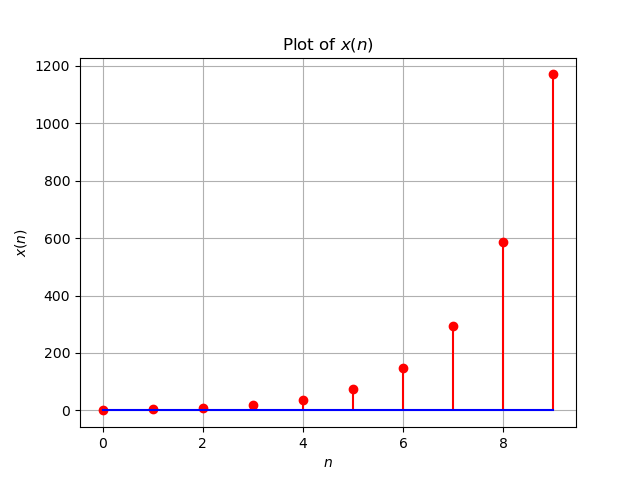
\includegraphics[width=\columnwidth]{fncert-maths/11/9/3/14/figs/plotx.png}
    \caption{stem plots of $x(n)$}
    \label{fig:11.9.3.14.1}
\end{figure}

\begin{figure}[h!]
    \centering
    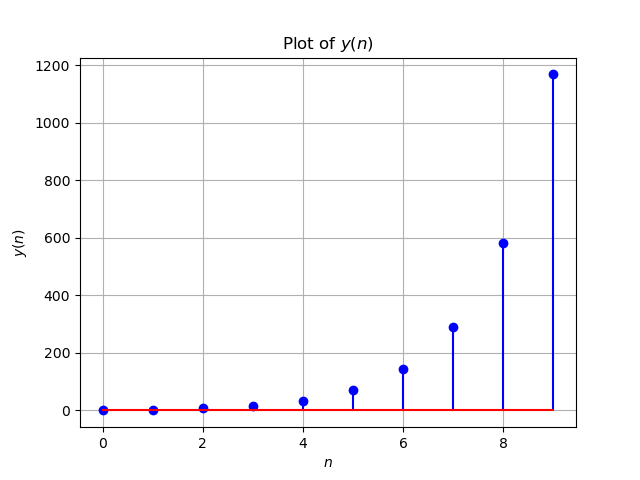
\includegraphics[width=\columnwidth]{ncert-maths/11/9/3/14/figs/plot.png}
    \caption{stem plots of $y(n)$}
    \label{fig:11.9.3.14.2}
\end{figure}

